\chapter{\telemacsystem{} development plan}
\label{devplan}

The development plan describes explicitly all the processes on the software
during the life cycle of the \telemacsystem{} code and insures its Quality.

The \telemacsystem{} activity is decomposed into three main activities that are
described in Chapter~\ref{devact}:
\begin{itemize}
\item \textbf{Development activity}.
\item \textbf{Verification and Validation activity}.
\item \textbf{Release activity}.
\end{itemize}

\section{Rights to commit new developments}

People intervening in the development of \telemacsystem{} can be divided in the
following groups:
\begin{itemize}
\item \textbf{The \telemacsystem{} development team (TDT)}: To be a part of the
  TDT you need to have writing access on the subversion repository. To be in
  the development team, the developer must have read the developer guide and
  the SQP in order to apply it to its future developments. The PM is a member
  of the TDT\@.
\item \textbf{Developers from EDF units}: They are developers from one of the
  group of EDF and are developing for the \telemacsystem{} project. It is
  recommended that they follow the \telemacsystem{} workshop. They will need to
  contact a member of the TDT to integrate their development.
\item \textbf{Non EDF developers working with EDF}: They can be subcontractors,
  interns, PhD students or any other partners working with EDF\@. It is also
  recommended that they follow the \telemacsystem{} workshop. The follow-up of
  the development will have to be done by a members of the TDT\@.
\item \textbf{Open source community, academic and industrial partners}:
  \telemacsystem{} is an open source code under GNU-GPL\@. Anyone can get the
  source and develop his own version. But for a development to be integrated in
  the official version, it must be studied by the TDT and follow the process
  described in~\ref{dev}. If the integration is validated, the delivery of the
  evolution for the code must go through a member of the TDT
  (See~\ref{devint}).
\end{itemize}

\section{Life cycle of a development}

\subsection{Definition of a development}
\label{defdev}

A development represents a modification on the source code of \telemacsystem{},
its documentation and its dedicated tools. (i.e.\ everything that is under the
configuration, see~\ref{conf}). The developments are categorised in three types
of maintenance:
\begin{itemize}
\item \textbf{Evolution maintenance}: This maintenance aims to upgrade the
  software in order to:
  \begin{itemize}
  \item Break limits of some existing functionalities (performance, strength,
    precision\ldots).
  \item Develops new functionalities to satisfy new needs or demands.
  \end{itemize}
  Those evolutions can be developments of new features made by one of EDF Units.
  They can also originate from an outside developer and been brought in by the
  PM\@.
  Every maintenance must be joined with a CUE ticket. This ticket will allow
  the PM to have a general view of the work in progress in the code. According
  to the size of the development, it can even be presented by the developer in
  an ADEPHE meeting, this will allow the TDT do evaluate the impact of the
  development and maybe advise the developer on what to do. The development
  must be validated by one of the CHs.
\item \textbf{Corrective maintenance}: The corrective maintenance is the
  removal of an anomaly in the code or the documentation. A bug can be:
  \begin{itemize}
  \item A problem in the code, a mistake in the documentation, an error in the
    GUI\@.
  \item An error in a test case detected during the Verification and Validation
    process.
  \item A problem in the implementation detected by user.
  \end{itemize}
  Corrective maintenance must also be coupled with a CUE ticket if that
  maintenance is also to applied for the current stable version.
\item \textbf{Adaptive maintenance}: The adaptive maintenance concerns
  evolution in the code to comply with a change of environment (Operating
  System, compiler, new cluster\ldots).
\end{itemize}

\subsection{Life cycle of a \telemacsystem{} development}
\label{lifecycle}
The life cycle of a \telemacsystem{} development follows a list of steps shown
on the Figure~\ref{cycle}. Those steps will be described in the next sections.

\begin{figure}[H]
\centering
\begin{tikzpicture}[node distance = 1cm, auto]
  % Defining style for the task
  \tikzstyle{task} = [draw, very thick, fill=white, rectangle]
  \tikzstyle{bigbox} = [draw, thin, rounded corners, rectangle]
  \tikzstyle{box} = [draw, thick, fill=white, rounded corners, rectangle]
  % Creation of the nodes
  \node (CUE) [task] {1. Ticket on CUE};
  \node (CHs) [task, below of=CUE] {2. CHs};
  \node (IMPL) [task, below of=CHs] {3. Implementation};
  \node (null2) [right of=IMPL, node distance=9em] {};
  \node (VV) [task, below of=IMPL] {4. Verification \& Validation};
  \node (DOC) [task, below of=VV] {5. Documentation};
  \node (INT) [task, below of=DOC] {6. Integration};
  \node (null1) [right of=INT, node distance=9em] {};
  \node (null3) [left of=INT, node distance=9em] {};
  \node (TRUNK) [box, below of=INT, node distance=4em] {Main branch of \telemacsystem{}};
  % big box
  \node (DEV) [bigbox, fit = (CUE) (CHs) (IMPL) (null1) (null2) (null3) (VV) (DOC) (INT)] {};
  \node at (DEV.north) [above, inner sep=3mm] {\textbf{Development}};
  % Creation of the path between the nodes
  \draw[->] (CUE) to node {} (CHs);
  \draw[->] (CHs) to node {} (IMPL);
  \draw[->] (IMPL) to node {} (VV);
  \draw[->] (VV) to node {} (DOC);
  \draw[->] (DOC) to node {} (INT);
  \draw[-] (INT) -- node [near start] {no} (null1.center);
  \draw[-] (null1.center) -- (null2.center);
  \draw[->] (null2.center) -- node [near start] {} (IMPL);
  \draw[->] (INT) to node {yes} (TRUNK);
\end{tikzpicture}
\caption{\label{cycle}Life cycle of a \telemacsystem{} development}
\end{figure}

Depending on the kind of development (corrective, adaptive, evolution
maintenance) some of those steps can be skipped.
The different steps are:
\begin{enumerate}
\item Proposal step.
\item Examination and impact study step.
\item Implementation step.
\item Verification step.
\item Documentation step.
\item Approbation and validation step.
\end{enumerate}

This development cycle is based on a V scheme life cycle, it contains those
different steps and the different types of testing (See next paragraph). To be
more precise it is more of spiral cycle in which the V cycle is read
iteratively in order to improve the quality gradually.

\section{Description of the development steps}
\label{dev}

\subsection{Proposal step}

Every demand must go through the proposal step may it be a corrective,
adaptive, evolution maintenance (See Section~\ref{defdev} for a definition).

This proposal is given to the TDT with a ticket on the CUE
(\url{cue.opentelemac.org}).

The goal of this proposal is to:
\begin{itemize}
\item Inform the CHs of the development proposed.
\item Give more information on the impact in the software.
\item Plan and organise the resources for the development.
\item To prepare the validation in ADEPHE if necessary.
\end{itemize}

\textbf{In charge}: The proposer.

\textbf{Documents}: The CUE ticket.

\subsection{Job repartition step}

When the cue ticket is published, the CHs have to determine if the development
must be followed by the TDT\@. This mainly concerns evolution maintenance but
can also concern corrective maintenance if it has a major impact on the code.

The goal of this step is:
\begin{itemize}
\item If it is an evolution maintenance, to verify the coherence of the
  evolution with: the kernel, the existing, in development or planned
  functionalities, the functionality itself, the modifications needed in the
  data structure, the architecture of the code or the GUI, the name of the new
  keywords and structure. In particular guiding the developer towards a reusing
  of existing routines.
\item In case of a corrective maintenance it studies the impact on the
  Validation and Verification process.
\item To help the developer in its choice of algorithm and implementation.
\item To discuss the test cases for Validation and Verification.
\item To estimate the impact on the documentation.
\end{itemize}

\textbf{In charge}: CHs, TDT, handler of the development.

\textbf{Documents}:
\begin{itemize}
\item Input: The CUE ticket.
\item Output: Update of evolution on the CUE ticket.
\end{itemize}


\subsection{Implementation step}

This is the coding part of what was specified in the CUE ticket, with the
modifications that the discussion during the ADEPHE could have generated.

The developer must follow the coding convention given in the developer guide of
\telemacsystem. All the developments are done under a configuration handling
tool, for each development a branch is created dedicated to that development.

The control of the implementation is made by running the \telemacsystem{}
validation. If possible for an evolution maintenance it is good to add a test
case that checks the new functionality if one does not exist.

The development must be done on a branch and follow the development version (or
trunk, see Section~\ref{conf} for a definition) using a configuration handling
tool. It is strongly recommended to keep up to date with the development
version as often as possible. This lessens the workload of that process
compared to doing it at the end of the development.

It is also recommended to use developing tools during the development like a
debugger (gdb, totalview), valgrind for memory leak.

The CUE ticket is updated as the implementation goes on.

\textbf{In charge}: The developer.

\textbf{Documents}:
\begin{itemize}
\item Input: CUE ticket, developer manual, verification and validation test cases.
\item Output: source code, test cases (with xml), results of tests.
\end{itemize}

\subsection{Verification step}

The Verification and Validation process is deeply linked with the
implementation process. This process aims to verify the code on the algorithm
level and the whole model using the Validation and Verification test cases
(even if a small part of the code was modified like during a corrective and
adaptive maintenance). This is then complementary (even redundant) with the
Verification done during the implementation. The Verification and Validation
are explained in Chapter~\ref{vv}.

As mentioned in the previous paragraph every development must contain
Validation and Verification test cases:
\begin{itemize}
\item Evolution maintenance: For an evolution of the code at least one
  Verification and one Validation case must be added if existing cases cannot
  be used. The choice of those cases are discussed with the TDT\@.
\item Corrective and adaptive maintenance: All the test cases must be rerun.
\end{itemize}

\textbf{In charge}: The developer.

\textbf{Documents}:
\begin{itemize}
\item Input: CUE ticket, validation manual, ticket for each case.
\item Output: update of CUE ticket, \LaTeX\xspace documentation follow the validation
standard for each test case.
\end{itemize}

\subsection{Documentation step}

The \telemacsystem{} technical documentation is composed of the following manuals:
The five below are duplicated for each \telemacsystem{} module.
\begin{itemize}
\item \textbf{Reference Manual}: describes every keyword in the dictionary of
  one module.
\item \textbf{Theory guide}: describes the physical phenomena modelled by the
  module and the numerical methods used to solve the equations modelling these
  phenomena.
\item \textbf{Validation Manual}: presents a list of test cases which validate
  the conceptual model, algorithms and software implementations. It is a
  concatenation of all the test case documentation for one module.
\item \textbf{User Manual}: describes how to use the code.
\end{itemize}

\begin{itemize}
\item \textbf{Online Manual (Doxygen)}: This documentation is linked with the
  source code (it is built by using special comment written in the source code),
  it describes the functions and structures of the source code.
\item \textbf{Developer Manual}: describes all the actions a developer might
  have to do during a development. It also defines the programming convention.
\item \textbf{NEWS.txt}: list for every release the new functionalities and the
  corrections.
\end{itemize}

The documentations are under configuration handler (svn) in \LaTeX\xspace
format. The documentation is under the responsibility of the Doc Handler and
the CHs.

Depending on the type of development a few cases can occur:
\begin{itemize}
\item \textbf{Evolution Maintenance}: For a new functionality of the code, a
  new section must be added in the theory guide describing the new physics and
  in the user manual showing how to use that functionality. The Online
  documentation must be updated as well. Update of the \textbf{NEWS.txt} with
  the new development.
\item \textbf{Corrective, adaptive Maintenance}: If the development has an
  impact on the documentation, it must be updated by the developer. If the
  development is to be merged on the version branch the \textbf{NEWS.txt}
  should be updated as well.
\end{itemize}

In any case the modification must go through the Doc Handler and must be
validated by the CHs and the PM\@.

\textbf{In charge}: The Doc Handler.

\textbf{Documents}:
\begin{itemize}
\item Input: All the documentation.
\item Output: The updated documentation.
\end{itemize}

\subsection{Integration step}

The integration step concerns the restitution of a development into the
main branch of the \telemacsystem{} (trunk, see~\ref{conf}).

The integration step is composed of the following steps:
\begin{itemize}
\item Designing the member of the TDT in charge of the integration of the
  development.
\item Integration of the verification and validation cases under the
  supervision of the V\&V Handler.
\end{itemize}

Not following those steps allows the CHs to refuse the integration and even
remove it from the development version.

\textbf{Presentation of the development in ADEPHE}

The ADEPHE meeting are monthly.
To be allowed in ADEPHE, a developer must have:
\begin{itemize}
\item Synchronized its branch with the latest version of the main branch
  (trunk).
\item Verified that the code follows the programming rules.
\item Added the new test cases for the development.
\item Validated his branch on the Validation tools (CIS).
\item Updated the CUE ticket.
\end{itemize}

During the ADEPHE the person in charge of the development must present:
\begin{itemize}
\item The development and how it was implemented: the functionalities if it is
  an evolution maintenance, in case of a corrective, adaptive maintenance: the
  data structure, the new keywords, how to use it.
\item The Verification and Validation cases and their results.
\item The impact on the documentation.
\end{itemize}

At the end of the presentation the TDT must decide:
\begin{itemize}
\item The integration or the dismissal of the development in the trunk.
\item The integration or the dismissal of the test case.
\item The integration or the dismissal of the modifications on the
documentation.
\item The person in charge of the integration.
\end{itemize}

In case of a disagreement in the TDT the PM has the final word.

\textbf{In charge}: CHs, TDT\@.

\textbf{Documents}:
\begin{itemize}
\item Input: CUE ticket, documentation.
\item Output: update of CUE ticket.
\end{itemize}

\textbf{Integration}

After the green light of the TDT the person in charge of the integration has to
do the following actions:
\begin{itemize}
\item Push the development and the documentation modifications into the \telemacsystem{}
main branch.
\item Integrate the Validation and Verification cases in the cases database.
\item Close the CUE ticket.
\end{itemize}

\textbf{In charge}: TDT\@.

\textbf{Documents}:
\begin{itemize}
\item Input: CUE ticket.
\item Output: update of CUE ticket, documentation, sources.
\end{itemize}

\subsection{Checklists for Developer and for Integrator}

To summarise the step that were explained before here is a checklist of the
actions he will have to do:
\begin{todolist}
\setlength\itemsep{0.01em}
\item Create a CUE ticket (on cue.opentelemac.org).
\item Discuss with TDT\@.
\item Do the work.
\item Update to the latest TRUNK version.
\item Update documentation.
\item Update \verb!NEWS.txt! with new feature.
\item Add test cases to test the development (with documentation, graphics and
  validation in the XML).
\item Run \verb!scripts/check_code.sh! (to check Fortran code convention).
\item Run \verb!pylint! (to check Python code convention).
\item Run \verb!compile_telemac.py --clean! for normal and debug configuration.
\item Run \verb!validate_telemac.py! for normal and debug configuration.
\item Run \verb!validate_telemac.py --notebook! for normal and debug configuration.
\item Run \verb!doc_telemac.py! if there are any modifications in the documentation.
\item Run \verb!damocles.py --eficas! if there are any modifications in the
  dictionaries.
\item Transmit development to the integrator.
\end{todolist}


The following checklist describes the actions that the integrator must follow:
\begin{todolist}
\setlength\itemsep{0.01em}
\item Check that the CUE ticket exist that it is properly filled.
\item Check that the code follows the coding convention.
\item Check that the test cases are appropriate.
\item Check that the implementation of the solution is good.
\item Check that the development is up to date with the trunk.
\item Check that the \verb!NEWS.txt! is updated.
\item Integrate the development into the TRUNK\@.
\end{todolist}


\section{Maintenance}

In this part the maintenance concerns only the corrective and adaptive maintenance.

The \telemacsystem{} project is in charge of the non-regression of the
\telemacsystem{} functionalities on the Verification and Validation test base.

The \telemacsystem{} project is also in charge of the adaptive maintenance (see
Section~\ref{defdev}).

The project in charge of other developments is in charge of the corrective
maintenance for their developments. But a help from the TDT is possible in
case of big difficulties. If the bug is easy to correct the TDT can, with the
authorisation of the person on charge, correct the bug themselves.

In any case the development must follow the development step described in
Section~\ref{lifecycle} and summarised in Figure~\ref{cycle}.

If the bug is also in the version branch it should also be merged there and a CUE
ticket must be created.

\textbf{Removal of a functionality}

The CHs can decide to remove a functionality if it has become obsolete or
irrelevant. This decision must be validated by the PM\@. The CHs must warn the
user community.

The removal of a functionality can only happen on the trunk, it is not
retroactive.

The removal of a functionality concerns:
\begin{itemize}
\item The source code and the library linked.
\item If there are any, the verification and validation impacted.
\item The documentation.
\end{itemize}

\section{Integration of development from the open-source community}
\label{devint}

An integration from the open-source community must follow the same process as
an internal development.

\section{Configuration handling}
\label{conf}

\subsection{Tools of configuration handling}

The different versions of the elements of the \telemacsystem{} software are
handled by a version control tool. Those tools allow to track the evolution and
ease the collaboration between multiple developers. Nonetheless, in addition to
those tools the source are backed up on the EDF network NOE\@.

The version control tool used is Subversion (SVN) which allows to rebuild any
version. The subversion repository is based at the following address:
\url{http://svn.opentelemac.org/svn/opentelemac}.

\subsection{Elements of the configuration}

The elements of the \telemacsystem{} software concerned by the configuration
control are the source code, the environment script, the documentation and the
test cases.

\subsection{Type of version}

\textbf{\telemacsystem{} official or reference version}

An official (or reference) version is a version handled by the \telemacsystem{}
project. The official version are:
\begin{itemize}
\item The version of exploitation.
\item The latest stable version, minor or major release.
\item The development version.
\end{itemize}

For example, the branch of development of the TDT are not considered
official.

\textbf{Creation of the reference version for \telemacsystem{}}

The creation of the reference version is described here:

The \telemacsystem{} version are handled using ``tags''.
\begin{itemize}
\item Creation of a tag is decided by the Chain Handler and the PM\@.
\item Tags are named in the format \textbf{vXpYrZ} where:
  \begin{itemize}
  \item \textbf{X} is the major version index, incremented when a major
    modification is done to the code (ex: makeover of the interface,
    modification of the code structure\ldots),
  \item \textbf{Y} is the minor version index, incremented when new minor
    functionalities are added to the software,
  \item \textbf{Z} is the patch index, incremented when a group of bug
    corrections are implemented in the software.
  \end{itemize}
\end{itemize}

The versions are divided into branches and tags. There is:
\begin{itemize}
\item \textbf{The main branch} (trunk), also called the development version. It
  represents the work in progress between two stable version. It is where the
  different maintenance are integrated. Figure~\ref{fig_lifecycle} shows the
  evolution of the main branch between two stable versions.
\item \textbf{The version branch} (\textbf{vXpY}), they are created every new
  major and minor version. They are used only for corrective and adaptive
  maintenance. They have been through the complete validation process. It is
  created in September.
\item \textbf{The stable version tag} (\textbf{vXpYrZ}), the tags are made from
  the version branch (\textbf{vXpY}) those tags are fixed they will not be
  modified. If a corrective or adaptive maintenance is necessary the changes
  will be made in the trunk and merged into the version branch and a new tag
  (\textbf{vXpYrZ+1}) will be created. Figure~\ref{fig_lifecycle} shows the
  creation of the \textbf{vXpY} and the tags created. The first tag is created
  (pending validation) two months after creation of the version branch.
\end{itemize}

\begin{figure}[H]
\centering
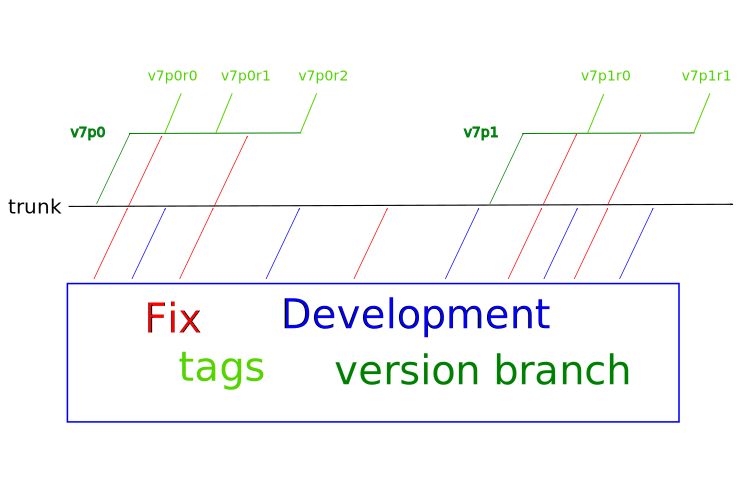
\includegraphics[scale=.5]{graphics/svn-cycle.pdf}
\caption{\label{fig_lifecycle}Life cycle of the \telemacsystem{} version}
\end{figure}

\subsection{Version schedule}

\textbf{Version release}

The different version major and minor are separated by a flexible interval:
\begin{itemize}
\item The major version are released every 4 to 5 years.
\item The minor version are released every year, if the amount of new
  development is considered acceptable.
\end{itemize}

Finally at any time we have the following versions:
\begin{itemize}
\item The development version: It is the main branch (trunk).
\item The latest stable version \textbf{vXpYrZ}.
\end{itemize}

This timetable can be modified due to a big change in the code that would
require longer validation to leave time for the normal integration to adapt.

\textbf{Removal of stable version}

The removal of a stable version is automatic when:
\begin{itemize}
  \item A corrective version \textbf{Z > 0} is released.
\item It reaches its expiration date.
\end{itemize}

\textbf{Version maintained}

Only last two minor versions are maintained.

\textbf{Exploitation version}

To do a study with \telemacsystem{} it is recommended to use the latest stable
version. It should be the most advanced and the one with less bugs.

\subsection{Checklist for version release}

Here is the actions that need to be done when creating a new version
\textbf{vXpY}\@:
\begin{todolist}
\setlength\itemsep{0.01em}
\item Create the branch \textbf{vXpY} from the trunk.
  \item Update the \verb!NEWS.txt!. Replace trunk section by section
    \textbf{vXpY}.
  \item In \verb!documentation/data/TelemacDocs.cls! change the command
    \verb!\telmaversion! to \textbf{vXpY}.
  \item In \verb!sources/utils/special/declarations_special.f! change the
    parameter VERSION to \textbf{vXpY}.
  \item In \verb!configs/systel.edf.cfg! change version to \textbf{vXpY}.
  \item Run \verb!validate_telemac.py!.
  \item Run \verb!validate_telemac.py --notebook!.
  \item Run \verb!doc_telemac.py!.
  \item Add all the generated documentation to repository.
  \item Run \verb!damocles.py --eficas!.
  \item Add the \verb!scripts/python3/eficas! folder to the repository.
\end{todolist}

Here are the actions that need to be done when creating a new version
\textbf{vXpYrZ}\@:
\input{latex/checklist_minor_release}
